% -*- mode: latex; -*- mustache tags:  
\documentclass[10pt,twoside,english]{_support/latex/sbabook/sbabook}
\let\wholebook=\relax

\usepackage{import}
\subimport{_support/latex/}{common.tex}

%=================================================================
% Debug packages for page layout and overfull lines
% Remove the showtrims document option before printing
\ifshowtrims
  \usepackage{showframe}
  \usepackage[color=magenta,width=5mm]{_support/latex/overcolored}
\fi


% =================================================================
\title{A PharoThings Tutorial}
\author{Allex Oliveira}
\series{Square Bracket tutorials}

\hypersetup{
  pdftitle = {A PharoThings Tutorial},
  pdfauthor = {Allex Oliveira},
  pdfkeywords = {IoT, Raspberry, PharoThings, Pharo}
}


% =================================================================
\begin{document}

% Title page and colophon on verso
\maketitle
\pagestyle{titlingpage}
\thispagestyle{titlingpage} % \pagestyle does not work on the first one…

\cleartoverso
{\small

  Copyright 2017 by Allex Oliveira.

  The contents of this book are protected under the Creative Commons
  Attribution-ShareAlike 3.0 Unported license.

  You are \textbf{free}:
  \begin{itemize}
  \item to \textbf{Share}: to copy, distribute and transmit the work,
  \item to \textbf{Remix}: to adapt the work,
  \end{itemize}

  Under the following conditions:
  \begin{description}
  \item[Attribution.] You must attribute the work in the manner specified by the
    author or licensor (but not in any way that suggests that they endorse you
    or your use of the work).
  \item[Share Alike.] If you alter, transform, or build upon this work, you may
    distribute the resulting work only under the same, similar or a compatible
    license.
  \end{description}

  For any reuse or distribution, you must make clear to others the
  license terms of this work. The best way to do this is with a link to
  this web page: \\
  \url{http://creativecommons.org/licenses/by-sa/3.0/}

  Any of the above conditions can be waived if you get permission from
  the copyright holder. Nothing in this license impairs or restricts the
  author's moral rights.

  \begin{center}
    
\includegraphics[width=0.2\textwidth]{_support/latex/sbabook/CreativeCommons-BY-SA.pdf}
  \end{center}

  Your fair dealing and other rights are in no way affected by the
  above. This is a human-readable summary of the Legal Code (the full
  license): \\
  \url{http://creativecommons.org/licenses/by-sa/3.0/legalcode}

  \vfill

  % Publication info would go here (publisher, ISBN, cover design…)
  Layout and typography based on the \textcode{sbabook} \LaTeX{} class by Damien
  Pollet.
}


\frontmatter
\pagestyle{plain}

\tableofcontents*
\clearpage\listoffigures

\mainmatter

\chapter{Lesson 9 - Ultrasonic Sensor (Distance)}
In the previous lessons, we learned how to control LEDs and to use a button to interact with LEDs. We learned also how to use the I2C sensors to read the temperature, humidity, pressure and x, y, z axis. Now let's use a different kind of sensor, that doesn't use I2C protocol. 
\section{What we need?}
In this lesson we will use a setup with 3 different I2C sensors.
\subsection{Components}
\begin{itemize}
\item 1 Raspberry Pi connected to your network (wired or wireless)
\item 1 Breadboard
\item 1 HC-SR04 sensor
\item 1 Resistor (1K ohms)
\item 1 Resistor (2K ohms)
\item Jumper wires
\end{itemize}
\section{Experimental theory}
Before constructing any circuit, you must know the parameters of the components in the circuit, such as their operating voltage, operating circuit, etc.
\subsection{The ultrasonic meassure}\subsection{How the HC-SR04 works?}\subsection{Limiting the return voltage with resistors}\section{Experimental procedure}
Now we will build the circuit. This circuit consists of 1 ultrasonic sensor HC-SR04, 1 resistor 1K ohms, 1 resistor 2K ohms and a power supply (the Rasp).

\begin{itemize}
\item Connect the Ground PIN from Raspberry in the breadboard blue rail (-). In this experiment we will use the PIN9 (Ground);
\item Then connect the 5V (PIN2) pin in the red rail (+). 
\item Now push the HC-SR04 sensor in the breadboard;
\item And insert the jumper wires connecting the sensor leg TRIG in the GPIO0 (PIN11) and the sensor leg ECHO in the breadboard, like the scheme showed in the Figure \ref{physicalSonicSensors};
\item Last step is to connect the power 5V and ground (-) wires from the breadboard rails in the sensor VCC + and GND (-) legs.
\end{itemize}

The Figure \ref{physicalSonicSensors} shows how the electric connection is made.


\begin{figure}

\begin{center}
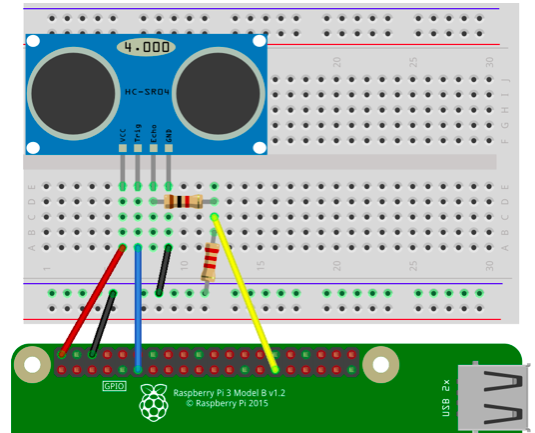
\includegraphics[width=0.6\textwidth]{/Users/allexoliveira/PharoThingsBook/Booklet-APharoThingTutorial/_result/pdf/Chapters/Chap10UltrasonicSensor/figures/pharothings-ultrasonic-board.png}\caption{Physical sensors connection.\label{physicalSonicSensors}}\end{center}
\end{figure}

\section{Connecting remotely}
Through your local Pharo image, let’s connect in the Pharo image by running on Raspberry, enable the auto-refresh feature of the inspector, and open the inspector.
Run this code in your local playground:

\begin{displaycode}{plain}
remotePharo := TlpRemoteIDE connectTo: (TCPAddress ip: #[193 51 236 212] port: 40423)
GTInspector enableStepRefresh.
remoteBoard := remotePharo evaluate: [ RpiBoard3B current].
remoteBoard inspect.
\end{displaycode}
\section{Experimental code}
In your inspect window (Inspector on a PotRemoteBoard), let’s create an instance of the ultrasonic sensor. 

\begin{displaycode}{plain}
d := board installDevice: PotHCSR04Device new. ​

\end{displaycode}

As we saw before, we can inspect the remote object to see some properties and methods. Let's use the method \textcode{readDistance} to read the distance: 

\begin{displaycode}{plain}
d readDistance. 

\end{displaycode}


% lulu requires an empty page at the end. That's why I'm using
% \backmatter here.
\backmatter

% Index would go here

\end{document}
